\chapter{Model predykcyjny}

\section{Definicja drzewa decyzyjnego}

Ocena ryzyka kredytowego, w tym przypadku predykcja, czy dana pożyczka będzie spłacana zgodnie z obowiązującymi terminami, jest typowym przykładem problemu klasyfikacji wektora danych w oparciu o dane historyczne. W tym celu implementowany system będzie wyposażony w moduł predykcyjny składający się z drzewa decyzyjnego wytrenowanego na wstępnie przetworzonych danych pobranych z serwisu Lending Club.

Drzewo decyzyjne to popularne narzędzie wykorzystywane przy wspomaganiu procesu decyzyjnego, często wykorzystywane w uczeniu maszynowym przy wydobywaniu wiedzy z danych historycznych. Ma ono charakter struktury drzewiastej \cite{MED}, składającej się z:

\begin{itemize}
	\item korzenia, czyli węzła wejściowego drzewa, zawierającego wszystkie dane,
	\item węzłów wewnętrznych zawierających testy na wartościach atrybutów, które określają podzbiór danych spełniających test (z każdego z tych węzłów wychodzi dokładnie tyle gałęzi, ile jest możliwych wyników tego testu),
	\item liści, czyli węzłów, które zawierają informację o klasyfikacji obiektów.
\end{itemize}
Rysunek \ref{tree:example} przedstawia przykładowe drzewo decyzyjne, przedstawiające proces podejmowania decyzji określającej, czy pogoda sprzyja wyjściu z domu, czy nie.

\begin{figure}[H] \centering %H if want to get it exaclty here
	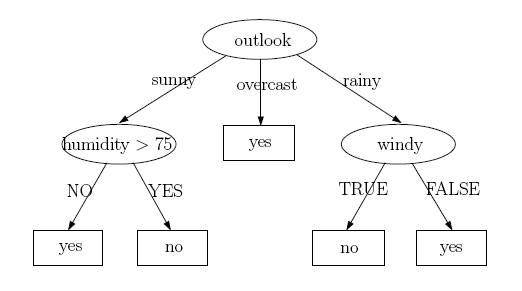
\includegraphics[scale=0.5]{img/decision_tree_example.png}
	\caption{Przykład drzewa decyzyjnego \cite{MED}.}
	\label{tree:example}
\end{figure}

Przy ocenie jakości drzewa należy wziąć pod uwagę następujące cechy \cite{treeMIMUW}:

\begin{itemize}
	\item rozmiar:
		\begin{itemize}
			\item liczba węzłów,
			\item wysokość,
			\item liczba liści,
		\end{itemize}
	\item dokładność klasyfikacji na zbiorze treningowym,
	\item dokładność klasyfikacji na zbiorze testowym.
\end{itemize}
Dobre drzewo decyzyjne charakteryzyje się nie tylko wysoką dokładnością klasyfikacji na zbiorach treningowym i testowym, ale także stosunkowo niewielkim rozmiarem.

\subsection{Konstrukcja drzew decyzyjnych}

Budowa drzewa przebiega w sposób rekurencyjny i składa się z następujących kroków \cite{PJWSTK}:

\begin{enumerate}
	\item Drzewo zaczyna od pojedynczego węzła reprezentującego cały zbiór treningowy.
	\item Jeżeli wszystkie przykłady należą do jednej klasy decyzyjnej, to zbadany węzeł staje się liściem i jest on etykietowany tą decyzją.
	\item W przeciwnym przypadku algorytm wykorzystuje miarę entropii (funkcja przyrostu informacji) jako heurystyki do wyboru atrybutu, który najlepiej dzieli zbiór przykładów treningowych.
	\item Dla każdego wyniku testu tworzy się jedno odgałęzienie i przykłady treningowe są odpowiednio rozdzielone do nowych węzłów (poddrzew).
	\item Algorytm działa dalej w rekurencyjny sposób dla zbiorów przykładów przydzielonych do poddrzew.
	\item Algorytm kończy się, gdy kryterium stopu jest spełnione.
\end{enumerate}
W sytuacji, kiedy dany zbiór składa się z obiektów przypisanych do różnych klas decyzyjnych, eytkietą staje się klasa o najliczniejszej reprezentacji.

Rysunek \ref{tree:algorithm} przedstawia pseudokod algorytmu budowy drzewa decyzyjnego. Kryterium stopu jest spełnione, gdy aktualny zbiór obiektów \cite{treeMIMUW}:

\begin{itemize}
	\item jest pusty,
	\item zawiera obiekty wyłącznie jednej klasy decyzyjnej,
	\item nie ulega podziałowi przez żaden test.
\end{itemize}


\begin{figure}[h] \centering %H if want to get it exaclty here
	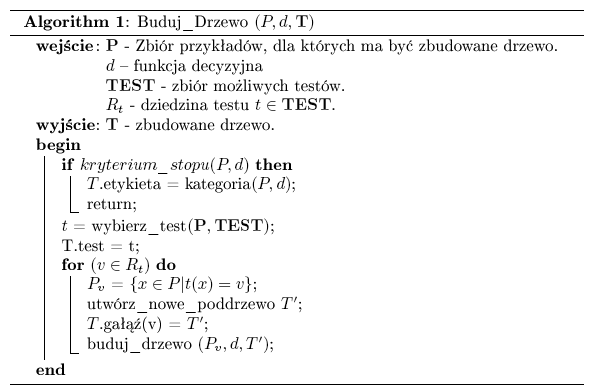
\includegraphics[scale=0.5]{img/tree_algorithm.png}
	\caption{Algorytm budowy drzewa decyzyjnego \cite{PJWSTK}.}
	\label{tree:algorithm}
\end{figure}

\section{Badanie modelu predykcyjnego}

Do budowy modelu predykcyjnego wykorzystano bibliotekę \textbf{party} języka skryptowego \textbf{R}. R jest popularnym narzędziem wykorzystywanym do analizy dużych zbiorów danych i badania pracy algorytmów uczenia maszynowego.

Zadaniem drzewa decyzyjnego będzie klasyfikacja pożyczki do jednej z dwóch klas - 0 lub 1, oznaczających odpowiednio pożyczkę spłaconą w terminie i pożyczkę niespłaconą lub spłaconą po wyznaczonym terminie.

\subsection{Model oparty na wszystkich zmiennych poddanych analizie}

Pierwsze badanie przeprowadzono z wykorzystyniem wszystkich zmiennych numerycznych poddanych analizie w poprzednim rozdziale, tj.:


\begin{itemize}
	\item $loan\_amnt$ - kwota kredytu,
	\item $int\_rate$ - stopa procentowa,
	\item $term$ - okres spłaty kredytu,
	\item $emp\_length$ - okres zatrudnienia kredytobiorcy,
	\item $annual\_inc$ - roczny przychód kredytobiorcy,
	\item $delinq\_2yrs$ - liczba rat, które nie zostały spłacone w terminie w ciągu ostatnich 2 lat,
	\item $dti$ - stosunek zadłużenia do przychodu kredytobiorcy,
	\item $paid\_amount\_ratio$ - stopień, w jakim kredyt został już spłacony.
\end{itemize}

Zgonie z przeprowadzoną analizą, zmiennymi na których powinny oparte być testy wygenerowane przez drzewo powinny być \textbf{int\_rate}, \textbf{term} oraz \textbf{paid\_amount\_ratio}.

W celu wykluczenia danych redundantnych przeprowadzono badanie korelacji pomiędzy poszczególnymi zmiennymi, które wykazało, że nie istnieje pomiędzy nimi zbieżność (Rysunek \ref{tree:correlation}).

\begin{figure}[h] \centering %H if want to get it exaclty here
	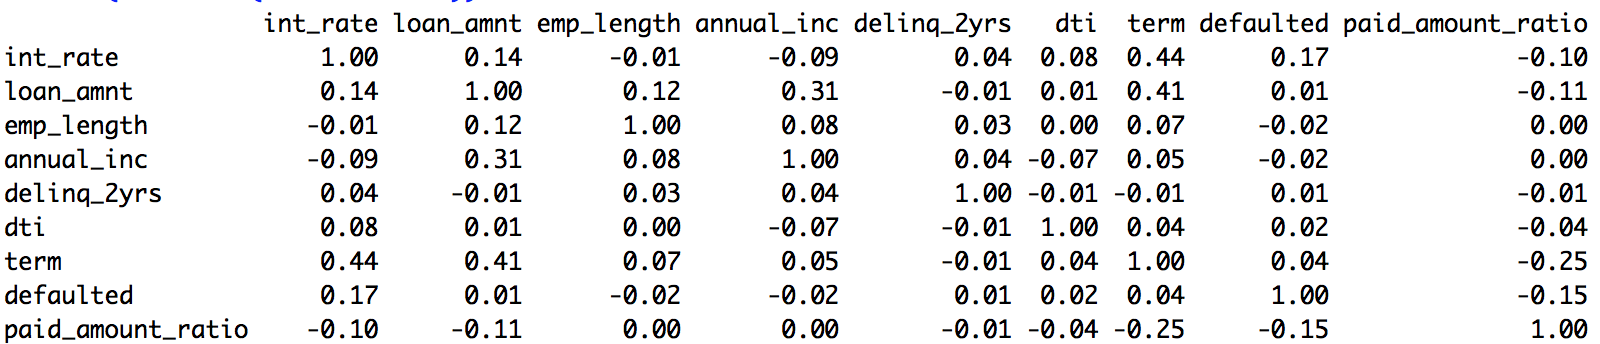
\includegraphics[scale=0.5]{img/tree_correlation.png}
	\caption{Macierz korelacji dla zmiennym wykorzystanych do budowy modelu drzewa decyzyjnego.}
	\label{tree:correlation}
\end{figure}

Następnie przeprowadzono podział zbioru danych na \textbf{treningowy}, \textbf{testowy} i \textbf{walidacyjny} w stosunku 7:2:1.

\begin{sidewaysfigure}
    \centering
    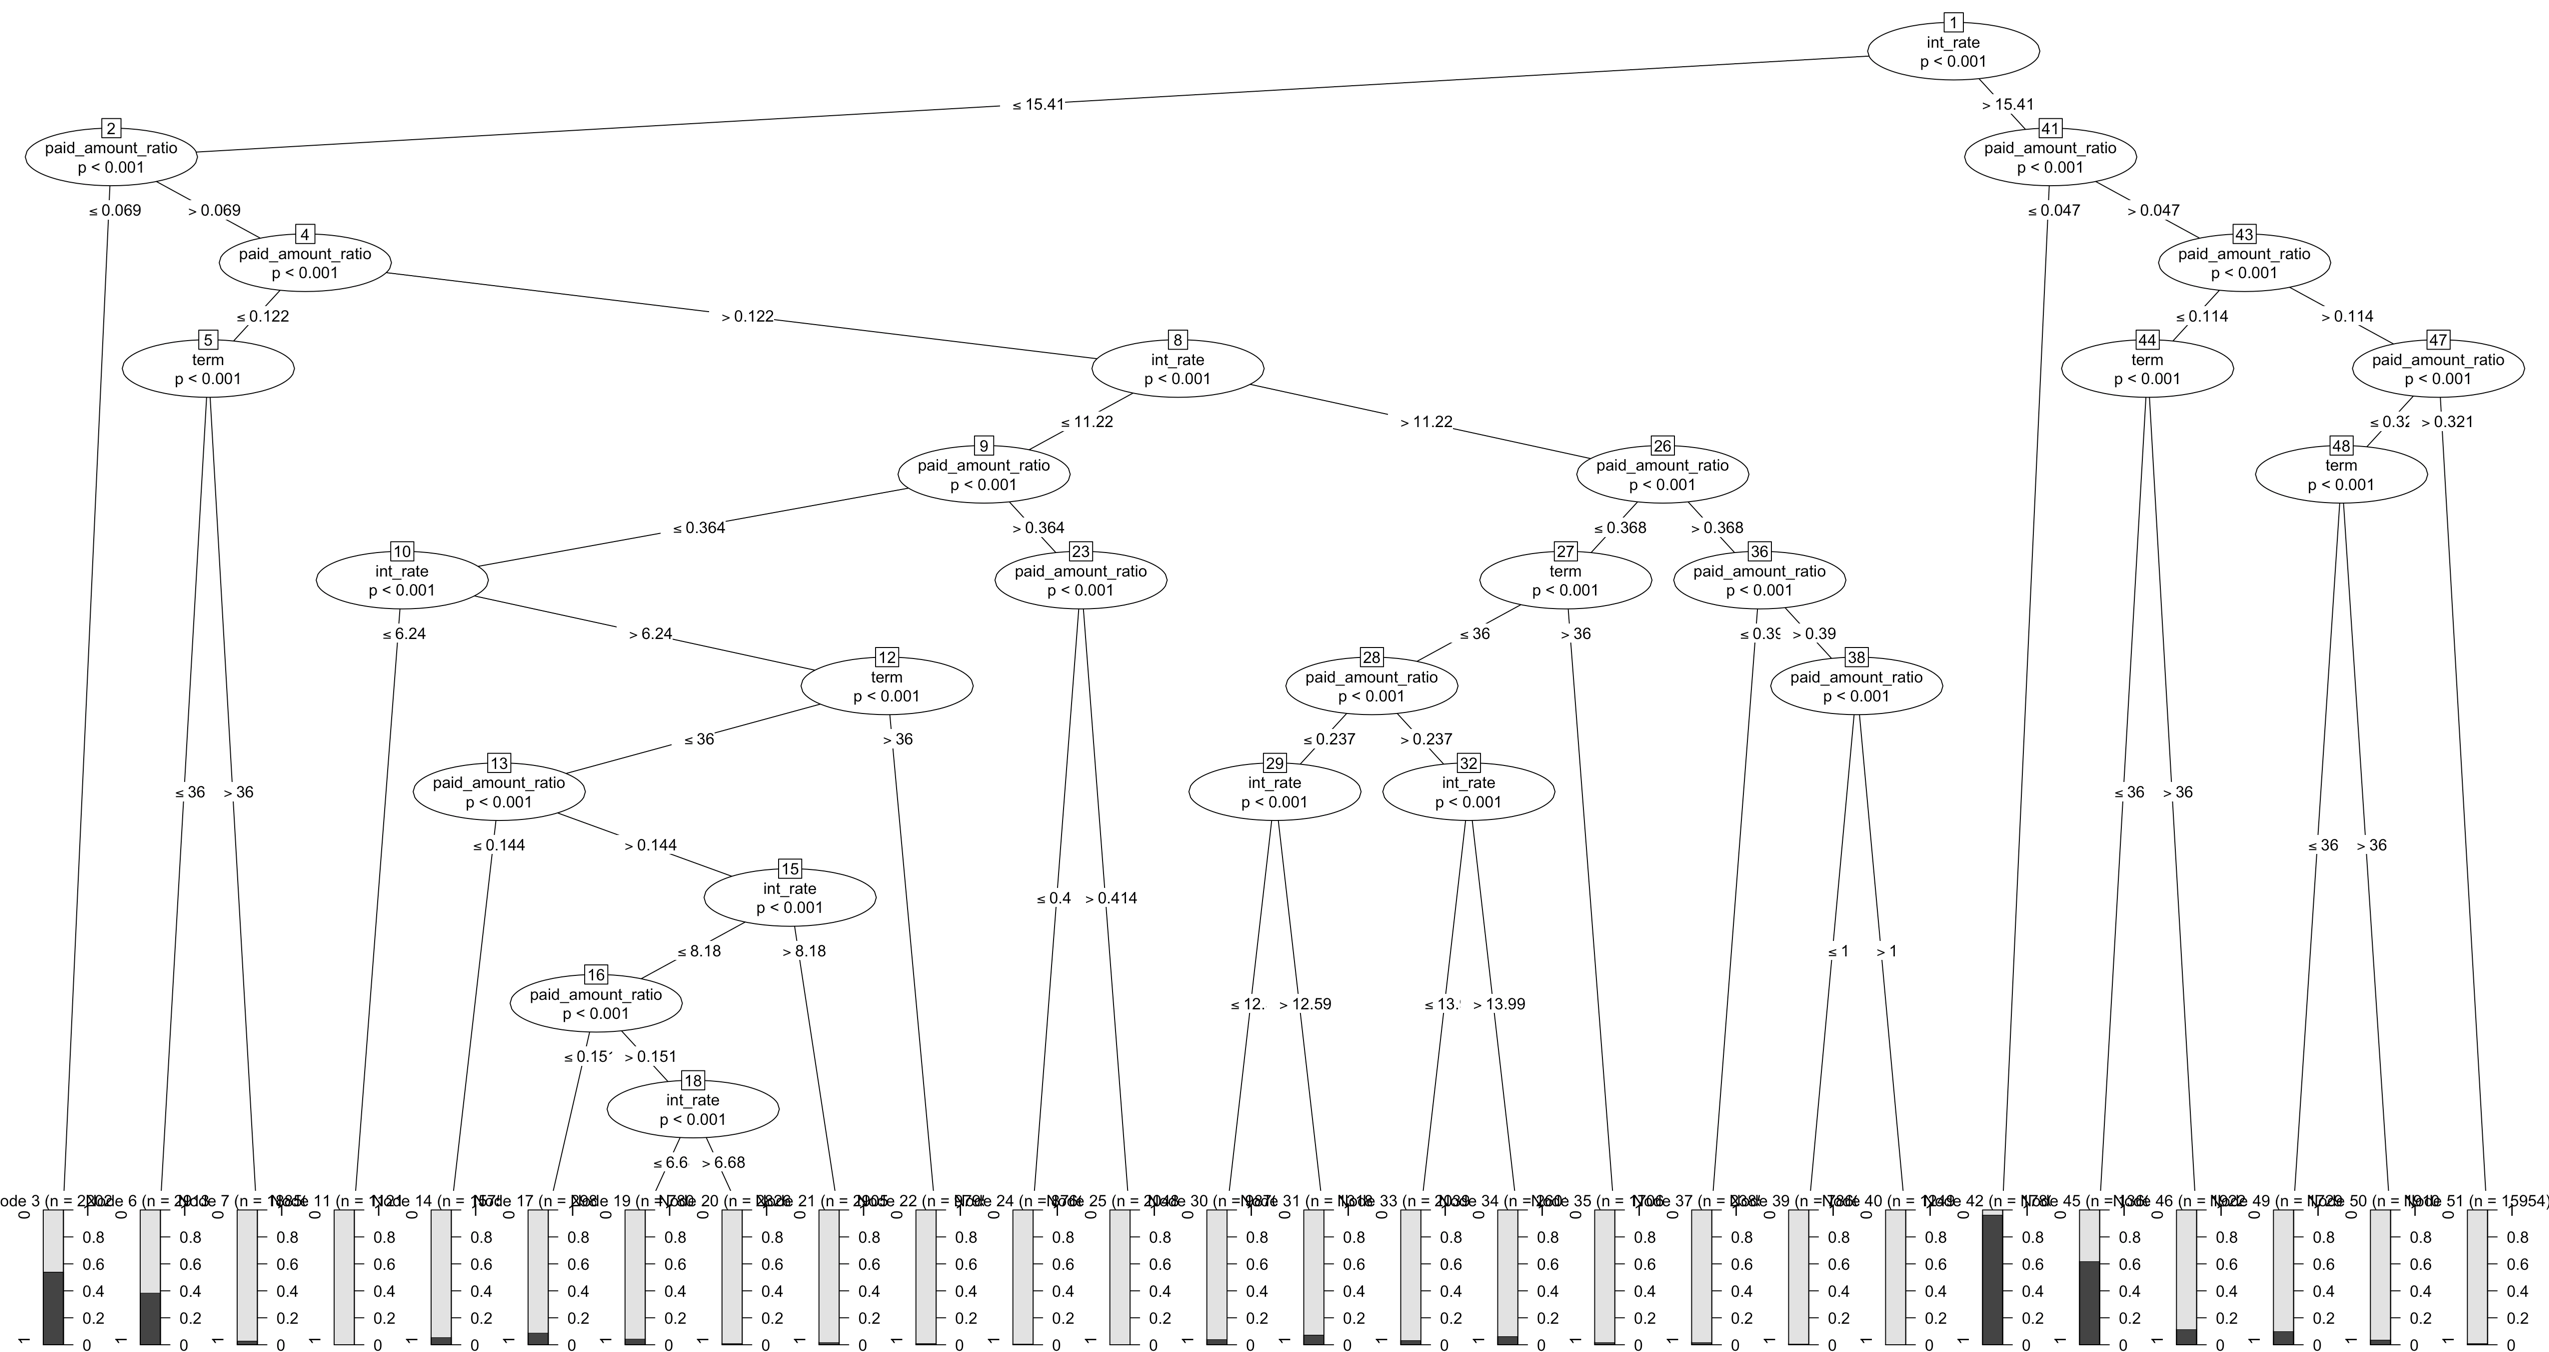
\includegraphics[scale=0.25]{img/tree_full.png}
    \caption{Drzewo decyzyjne uzyskane dla pełnego zakresu zmiennych.}
    \label{tree:full}
\end{sidewaysfigure}

Zgodnie z wynikami przeprowadzonej w poprzednim rozdziale analizy zbioru danych, uzyskany model korzystał jedynie ze zmiennych $int\_rate$, $term$ oraz $paid\_amount\_ratio$ przy tworzeniu kolejnych węzłów (Rysunek \ref{tree:full}) - pozostałe atrybuty mogą zostać pominięte w dalszych badaniach.

Po zbadaniu jakości klasyfikacji na zbiorach testowym i walidacyjnym, uzyskano macierze pomyłek (Tabele \ref{tab:test_full} i \ref{tab:valid_full})wskazujące odpowiednio na 95,04\% i 95,84\% dokładność klasyfikacji, definiowanej jako odsetek poprawnie sklasyfikowanych obiektów.

\begin{table}[h]
\centering 
\setlength\tabcolsep{4pt}
\begin{minipage}{0.48\textwidth}
\centering
\begin{tabular}{|c|r|r|}\hline
\backslashbox{Klasa}{Wynik}
&\makebox[3em]{0}&\makebox[3em]{1}\\\hline\hline

0 & 79545 & 3061 \\ \hline
1 & 498 & 1114 \\	\hline

\end{tabular}
 \caption{Macierz pomyłek dla drzewa decyzyjnego wykorzystującego wszystkie zmienne - zbiór testowy.} 
 \label{tab:test_full}  
\end{minipage}%
\hfill
\begin{minipage}{0.48\textwidth}
\centering
\begin{tabular}{|c|r|r|}\hline
\diagbox{Klasa}{Wynik}
&\makebox[3em]{0}&\makebox[3em]{1}\\\hline\hline

0 & 39802 & 1523 \\ \hline
1 & 228 & 556 \\ \hline

\end{tabular}
 \caption{Macierz pomyłek dla drzewa decyzyjnego wykorzystującego wszystkie zmienne - zbiór walidacyjny.} 
 \label{tab:valid_full} 
\end{minipage}
\end{table}

\subsection{Modele oparte na ograniczonej liczbie zmiennych}

Następnie zbadano modele, w których ogranioczono zbiór zmiennych, które wykorzystano do procesu uczenia. W pierwszej próbie wykorzystano zmienne, które zostały wskazane w wyniku analizy danych przeprowadzonej w poprzednim rozdziale. Uzyskany model (Rysunek \ref{tree:adjusted}) charakteryzuje się mniejszą liczbą węzłów i liści niż poprzedni, oraz większą dokładnością klasyfikacji, na co wskazują uzyskane macierze pomyłek (Tabele \ref{tab:test_adj} i \ref{tab:valid_adj}). Dokładność dla zbioru testowego i walidacyjnego wyniosła odpowiednio 95,66\% i 95,73\%, a liczba węzłów drzewa spadła o 59\% (z 51 do 21) - co z godnie z kryteriami ocenu jakości drzewa decyzyjnego opisanymi na początku tego rozdziału pozwala stwierdzić poprawę jakości modelu.

\begin{sidewaysfigure}
    \centering
    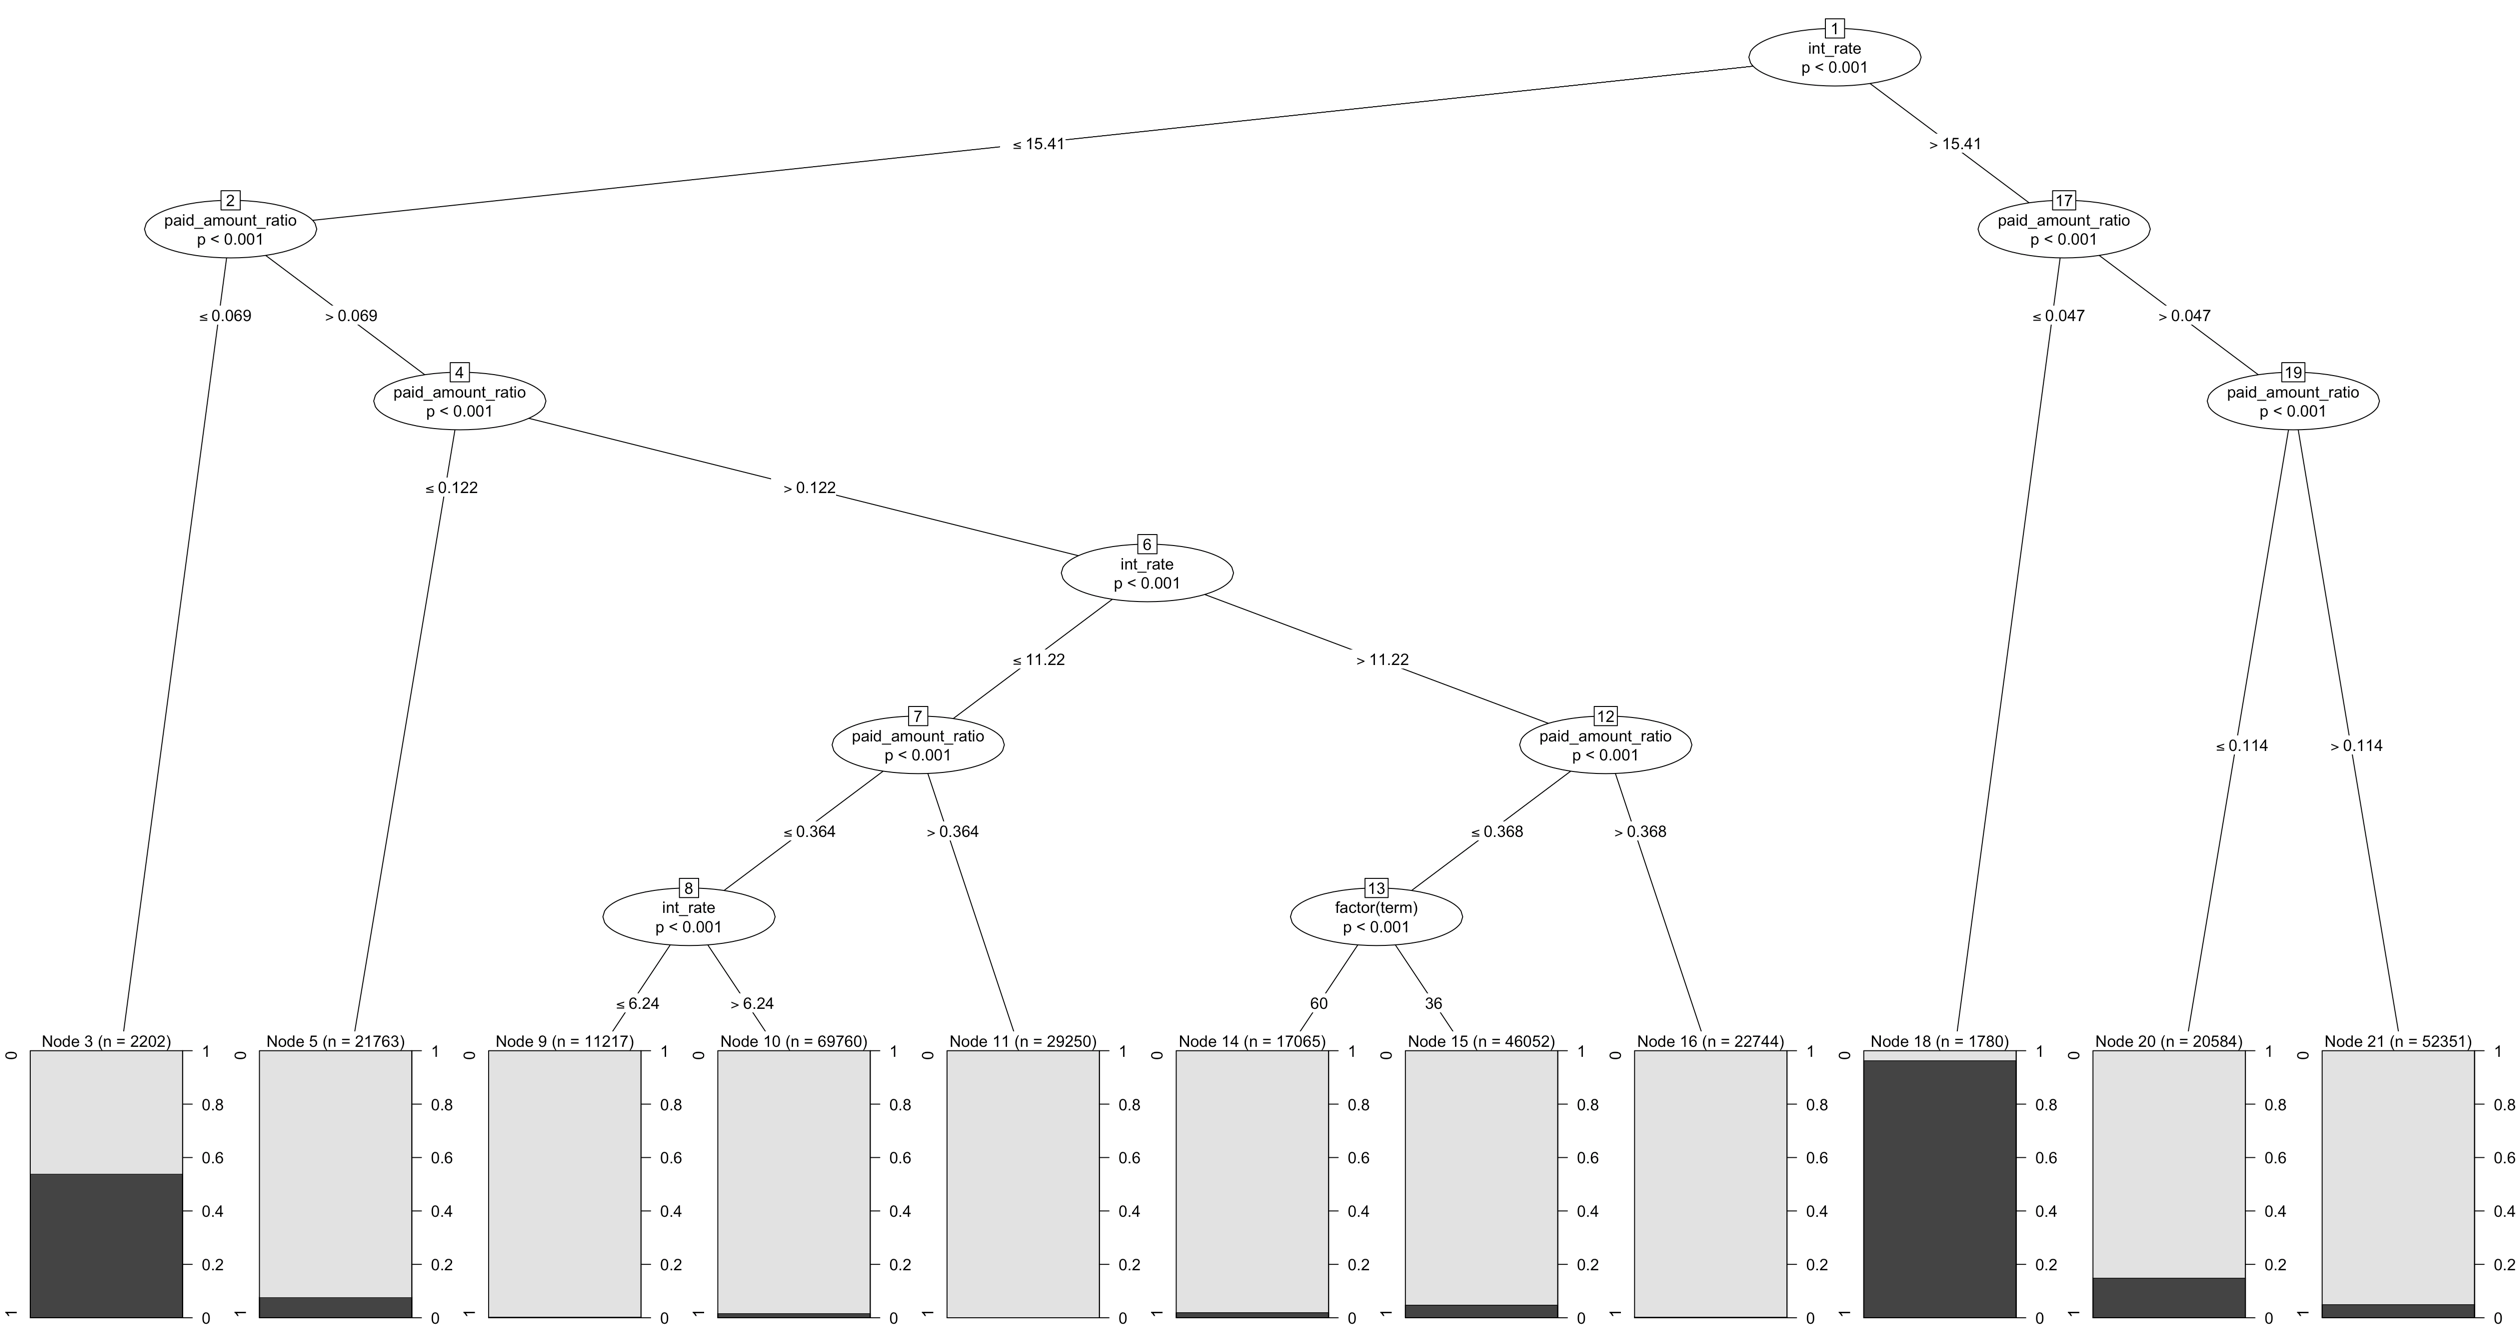
\includegraphics[scale=0.25]{img/tree_adjusted.png}
    \caption{Drzewo decyzyjne uzyskane dla ograniczonego zakresu zmiennych.}
    \label{tree:adjusted}
\end{sidewaysfigure}


\begin{table}[h]
\centering 
\setlength\tabcolsep{4pt}
\begin{minipage}{0.48\textwidth}
\centering
\begin{tabular}{|c|r|r|}\hline
\backslashbox{Klasa}{Wynik}
&\makebox[3em]{0}&\makebox[3em]{1}\\\hline\hline

0 & 79698 & 3306 \\ \hline
1 & 345 & 869 \\	\hline

\end{tabular}
 \caption{Macierz pomyłek dla drzewa decyzyjnego wykorzystującego ograniczony zbiór zmiennych - zbiór testowy.} 
 \label{tab:test_adj}  
\end{minipage}%
\hfill
\begin{minipage}{0.48\textwidth}
\centering
\begin{tabular}{|c|r|r|}\hline
\diagbox{Klasa}{Wynik}
&\makebox[3em]{0}&\makebox[3em]{1}\\\hline\hline

0 & 39882 & 1650 \\ \hline
1 & 148 & 429 \\ \hline

\end{tabular}
 \caption{Macierz pomyłek dla drzewa decyzyjnego wykorzystującego ograniczony zbiór zmiennych - zbiór walidacyjny.} 
 \label{tab:valid_adj} 
\end{minipage}
\end{table}

Ostatnim krokiem przy doborze modelu było sprawdzenie wyników dla poszczególnych par zmiennych. Okazało się, że najlepsze rezultaty uzyskano dla pary zmiennych $paid\_amount\_ratio$ i $term$. Otrzymane drzewo (Rysunek \ref{tree:final}) pozwoliło na redukcję liczby węzłów o 19\% w stosunku do poprzedniego (z 21 do 17) oraz o 67\% w stosunku do pierwotnego drzewa (z 51 do 21). Dokładność klasyfikacji również uległa poprawie - zarówno dla zbioru testowego jak i walidacyjnego wyniosła 95,9\% (Tabele \ref{tab:test_final} i \ref{tab:valid_final})

\begin{sidewaysfigure}
    \centering
    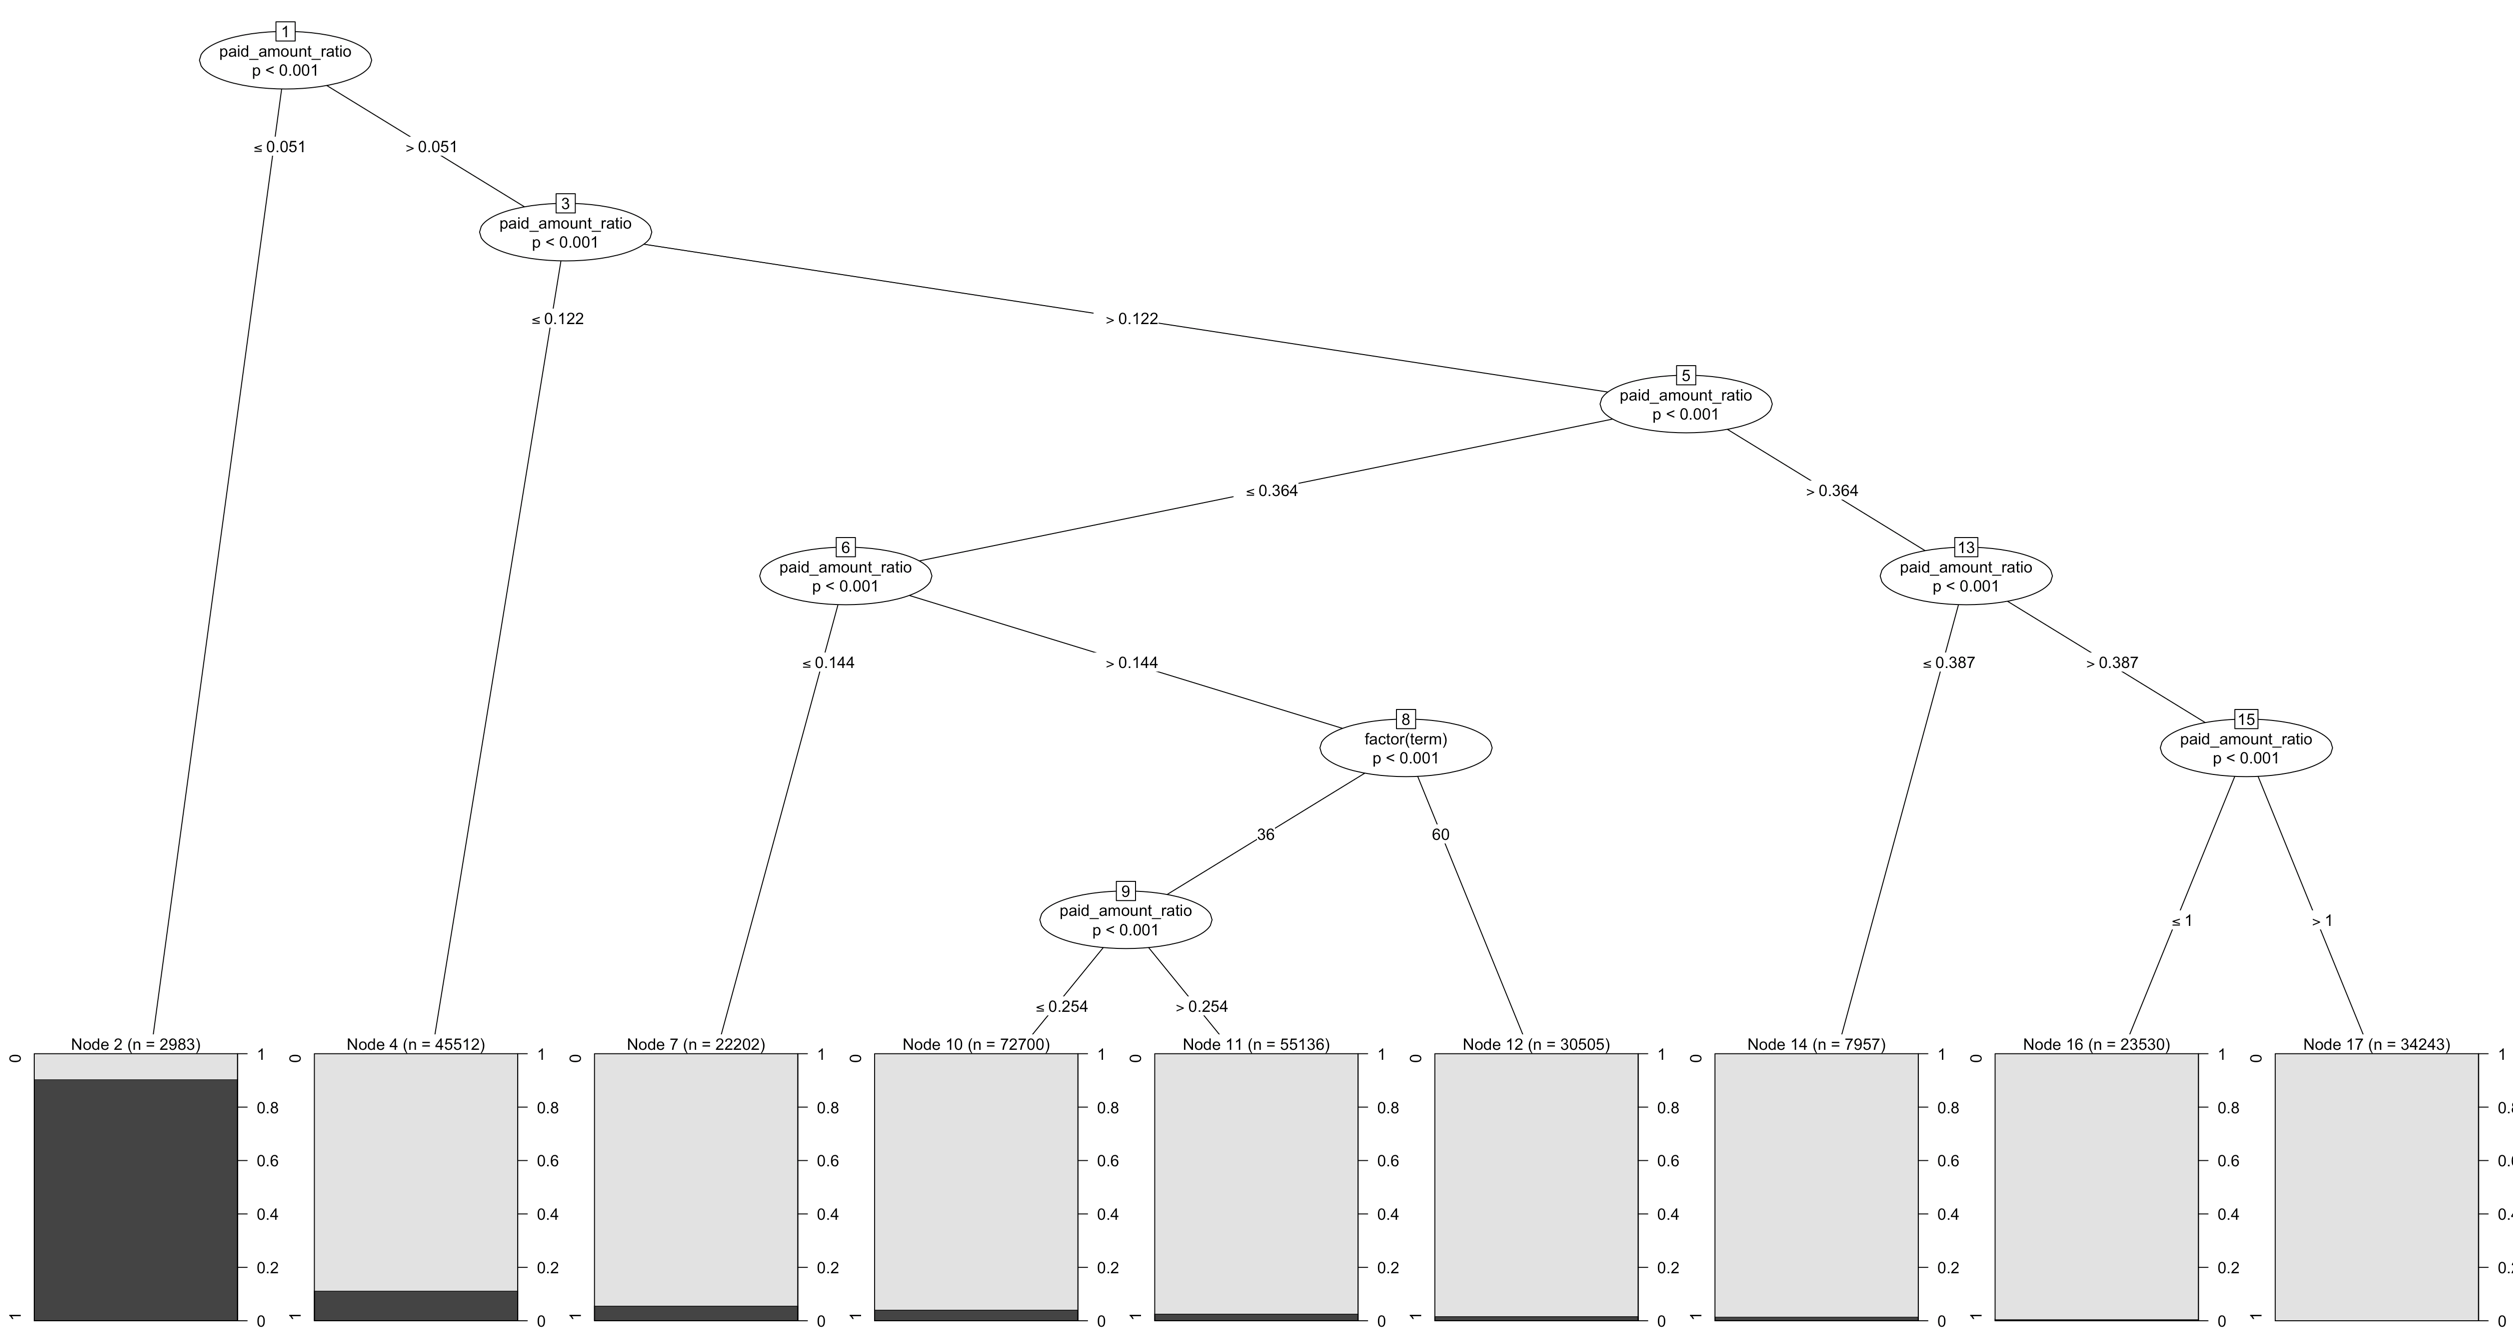
\includegraphics[scale=0.25]{img/tree_final.png}
    \caption{Najlepsze uzyskane drzewo decyzyjne.}
    \label{tree:final}
\end{sidewaysfigure}

\begin{table}[h]
\centering 
\setlength\tabcolsep{4pt}
\begin{minipage}{0.48\textwidth}
\centering
\begin{tabular}{|c|r|r|}\hline
\backslashbox{Klasa}{Wynik}
&\makebox[3em]{0}&\makebox[3em]{1}\\\hline\hline

0 & 79966 & 3372 \\ \hline
1 & 77 & 803 \\	\hline

\end{tabular}
 \caption{Macierz pomyłek dla najlepszego uzyskanego drzewa decyzyjnego - zbiór testowy.} 
 \label{tab:test_final}  
\end{minipage}%
\hfill
\begin{minipage}{0.48\textwidth}
\centering
\begin{tabular}{|c|r|r|}\hline
\diagbox{Klasa}{Wynik}
&\makebox[3em]{0}&\makebox[3em]{1}\\\hline\hline

0 & 39997 & 1683 \\ \hline
1 & 33 & 396 \\ \hline

\end{tabular}
 \caption{Macierz pomyłek dla najlepszego uzyskanego drzewa decyzyjnego - zbiór walidacyjny.} 
 \label{tab:valid_final} 
\end{minipage}
\end{table}

Badania przeprowadzone na drzewach decyzyjnych potwierdzają wyniki analizy przeprowadzonej w poprzednim rozdziale. Okazało się, że zmiennymi które mają wpływ na klasyfikację pożyczek pod względem ich zachowania są $int\_rate$, $term$ oraz $paid\_amount\_ratio$, a szczególnie dwie ostatnie. Ze względu na najwyższą dokładność i jednocześnie najmniejszą liczbę węzłów, w aplikacji zostanie wykorzystany ostatni z badanych modeli.